
\chapter{Single top quark production with a photon in the Standard Model}
\section{A brief overview of the standard model}

The standard model (SM) of particle physics, a so-called "gauge theory",  describes today's best knowledge of elementary physics. 
In the SM, there are two groups of particles and three fundamental forces of nature: the electromagnetic force, the strong nuclear force and the weak nuclear force. 
Every force coincides with an elementary particle, called a boson that acts as a force carrier. The second group of particles, the fermions, only interact with these force-carrying bosons if they have specific values for their quantum numbers.

The fermions have spin $s = \frac{1}{2} \hbar$ and can be divided into two separate groups. The first group, named quarks, are colour charge carrying fermions. 
There are three up-type quarks (up, strange and truth) with an electric charge of $q = +\frac{2}{3}e$ and three down-type quarks (down, charm and beauty) with an electric charge of $q = -\frac{1}{3}e$. 
The second group are the leptons. Three leptons have an electric charge of $q = +1e$. Furthermore, each of these leptons has a corresponding uncharged lepton partner called a neutrino.
Three different families further categorize leptons and quarks. These families are ordered by mass and consist of an up-type quark, the corresponding down-type quark, a lepton and the corresponding neutrino. 
There is an anti-matter particle equivalent for all fermions where every charge-like quantum number has the opposite sign. 

Particles with integer spin are called bosons. The SM lists four different bosons, called gauge bosons, with spin $s = 1$: $gluons$, $photons$, $Z$ and $W^{\pm}$. The Higgs boson is the only boson with spin $s=0$.
Gluons are colour charged and responsible for the strong nuclear force. They only couple to colour charged particles, including themselves. Photons carry the EM force to electrically charged particles. The massive bosons, $Z$ and $W^{\pm}$ are responsible for the weak nuclear force. They couple to particles with isospin. The weak force is the only way that neutrinos can interact with matter. Additionally, the $W^{\pm}$ boson is electrically charged, $q = \pm 1e$, and changes the flavour of a quark when coupling to it.
The Higgs boson explains how particles have mass. The boson arises from the electroweak symmetry theory and gives mass to particles via the Higgs mechanism. The interaction with the Higgs field is purely a product of electroweak symmetry breaking and is therefore not considered one of the fundamental forces.

A summary of the elementary particles in the standard model is given in \ref{fig:standard_model}.

\begin{figure}
    \centering
    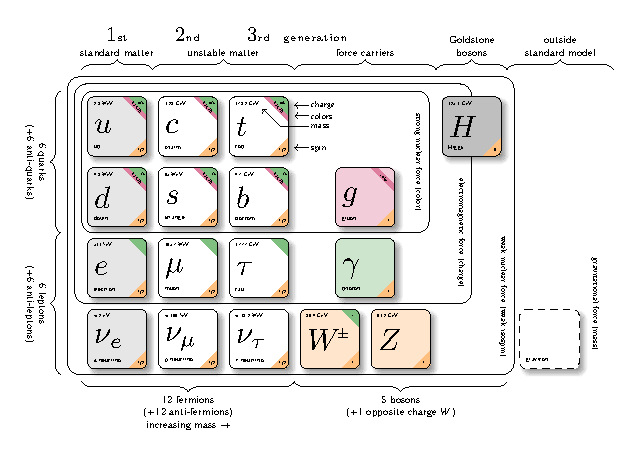
\includegraphics[width=0.9\textwidth]{Plots/model-physics.pdf}
    \caption{Elementary particles of the standard model alongside their propertie \cite{sm_table}.}
    \label{fig:standard_model}
\end{figure}

\section{The \texorpdfstring{$tq\gamma$}{tqGamma} process in the standard model}


The top quark (or truth quark) is an up-type quark and the most massive quark of the standard model with a mass of $m_t = 173.76 \pm 0.3 \,\si{\giga\electronvolt} (S =1.2)$ \cite{pdg}. It sometimes to a photon due of it's $q = +\frac{2}{3}e$ electric charge. 
In addition, the top quark has a colour charge and can therefore couple to gluons. The quark also interacts weakly because of its isospin of $I_z = +\frac{1}{2}$. Finally, the top quark has a very short decay width of $\Gamma = 1.42^{+0.19}_{-0.15} \,\si{\giga\electronvolt} (S=1.4)$ \cite{pdg} because of its high mass.
For this reason, top quarks cannot build any bound states and always decay shortly after production. Top quarks are therefore never observed directly. Instead, only their decay products are observable and can be retraced back to the top quark. 

The first discovery of the top quark was made at the Tevatron in 1995 during a proton-antiproton collision experiment (CITE). In 2009, the D0 \cite{singletop1} and CDF \cite{singletop2} collaborations also separately confirmed the measurement of the single-top-quark-process (tq) of the standard model at the Tevatron. The combined results are available in Ref. \cite{singletop3}. 
The CMS experiment at the LHC found evidence for the single-top-quark-process with an additional photon (tqGamma) with a standard deviation of $\sigma = 4.4$. The fiducial cross section 
was measured to be $\sigma(pp\rightarrow tq\gamma)(t\rightarrow\mu \nu b) = 115 \pm 17 (stat) \pm 30 (syst) \,\si{\femto\barn}$ for transverse momentum $p_T^\gamma > 25 \,\si{\giga\electronvolt}$ (CITE). (ADD BJÖRN PAPER REFERENCE). 

For the tqGamma-process, one gluon provided by the protons (also called parton) produces a bottom-antibottom-quark pair. The bottom quark then exchanges a W-boson with an arbitrary quark-parton, turning the bottom quark into a top quark and changing the flavour of the quark-parton. This top-quark then sends out a photon. 
The decay mode of the top quark follows this process. Top quarks decay by emitting a $W^+$-boson and turning into a bottom quark. The $W^+$-boson then decays shortly after into an antilepton and neutrino pair or a quark-antiquark pair of opposite types.

In Figure \ref{fig:feyn_tqGamma} the Feynman-diagram for the single-top+photon production is drawn. 
\begin{figure}
    \centering
    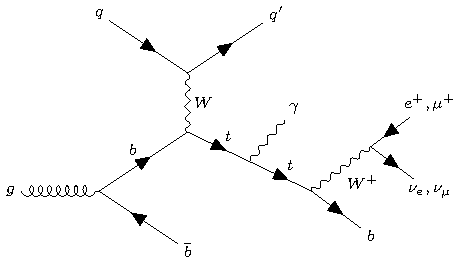
\includegraphics[width=0.9\textwidth]{Plots/s4_feyn_nom.pdf}
    \caption{Feynman diagram of the $tq\gamma$-process in the standard model.}
    \label{fig:feyn_tqGamma}
\end{figure}